\section{Formula Cheat Sheet}

\begin{minipage}[c]{0.4\textwidth}
Cross product:\quad
$\mathbf{a} \times \mathbf{b}=\left[\begin{array}{l}
a_{2} b_{3}-a_{3} b_{2} \\
a_{3} b_{1}-a_{1} b_{3} \\
a_{1} b_{2}-a_{2} b_{1}
\end{array}\right]$
\end{minipage}
\hfill
\begin{minipage}[c]{0.12\textwidth}
Trigonometric Identities:
\end{minipage}
\hfill
\begin{minipage}[c]{0.4\textwidth}
$$\begin{aligned}
&\sin(\alpha)^2 + \cos(\alpha)^2 = 1 \\
&\sin (\alpha\pm\beta)=\sin \alpha \cos \beta\pm\cos \alpha \sin \beta \\
&\cos (\alpha\pm\beta)=\cos \alpha \cos \beta\mp\sin \alpha \sin \beta \\
\end{aligned}$$
\end{minipage}
Determinant:

\begin{minipage}[c]{0.25\textwidth}
$$
|A|=\left|\begin{array}{ll}
a & b \\
c & d
\end{array}\right|=a d-b c .
$$
\end{minipage}
\hfill
\begin{minipage}[c]{0.7\textwidth}
$$
\begin{aligned}
|A|=\left|\begin{array}{lll}
a & b & c \\
d & e & f \\
g & h & i
\end{array}\right| &=a\left|\begin{array}{ll}
e & f \\
h & i
\end{array}\right|-b\left|\begin{array}{cc}
d & f \\
g & i
\end{array}\right|+c\left|\begin{array}{cc}
d & e \\
g & h
\end{array}\right| \\
&=a e i+b f g+c d h-c e g-b d i-a f h
\end{aligned}
$$
\end{minipage}
A manipulator may have special configurations, called ``isotropic points'', that are characterized by the Jacobi matrix having orthogonal columns of equal length, thus $J^{T} J=\delta I$ for some $\delta \in \mathbb{R}$.

\subsection{Denavit-Hartenberg Parameters}

\begin{minipage}[c]{0.1\textwidth}
DH-table (link-index $i$):
\end{minipage}
\hfill
\begin{minipage}[l]{0.25\textwidth}
\begin{tabular}{ |c|c|c|c|c| } 
\hline
$i$ & $a_{i-1}$ & $\alpha_{i-1}$ & $d_i$ & $\theta_i$ \\
\hline
1 & ... & ... & ... & ... \\ 
\hline
... & ... & ... & ... & ... \\ 
\hline
\end{tabular}
\end{minipage}
\hfill
\begin{minipage}[c]{0.6\textwidth}
\begin{center}
\begin{enumerate}
	\item Shift $Z_{i-1}$ by $a_{i-1}$ along $X_{i-1}$.
	\item Rot.\ $Z_{i-1}$ by $\alpha_{i-1}$ about $X_{i-1}$ \& shift by $d_i$ along $Z_i$.
	\item Rot.\ $X_{i-1}$ by $\theta_i$ about $Z_{i}$ \& move it to $Z_i$.
\end{enumerate}
\end{center}
\end{minipage}
\begin{center}
	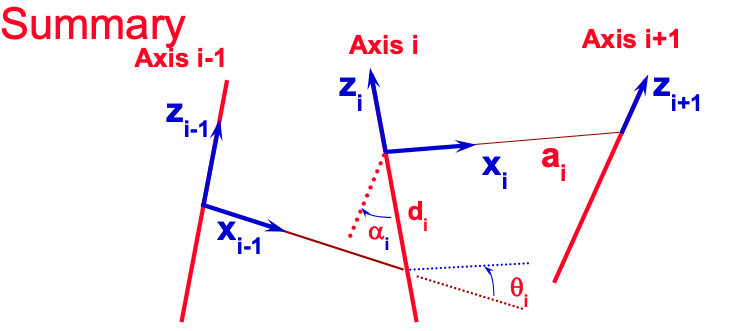
\includegraphics[width=7cm]{sections/imgs/2_dh_params.png}
	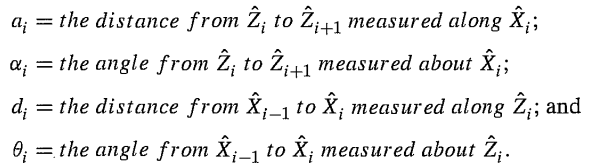
\includegraphics[width=9cm]{sections/imgs/11.png}
\end{center}
Homogeneous transformation from link $i$ to $i-1$:\quad	${ }^{i-1}_iT=\left[\begin{array}{ccc|c}
c \theta_{i} & -s \theta_{i} & 0 & a_{i-1} \\
s \theta_{i}\ c \alpha_{i-1} & c \theta_{i}\ c \alpha_{i-1} & -s \alpha_{i-1} & - s \alpha_{i-1}\ d_{i} \\
s \theta_{i}\ s \alpha_{i-1} & c \theta_{i}\ s \alpha_{i-1} & c \alpha_{i-1} & d_{i}\ c \alpha_{i-1} \\
\hline 0 & 0 & 0 & 1
\end{array}\right]$.\\
Inverse of the homogeneous transform:\quad	${ }^{A}_BT^{-1}={ }^{B}_AT=\left[\begin{array}{ccc|c}
 & {}^{A}_BR^T & & -{}^{A}_BR^T {}^AP_{Borg} \\
\hline 0 & 0 & 0 & 1
\end{array}\right]$.

\subsection{Jacobian}

\textit{Singularity}: the end-effector locally looses at least 1 DOF. This happens, when $Z$-axes are aligned $\Leftrightarrow$ the Jacobian does not have full rank $\Leftrightarrow det(J)=0$. Small end-effector motions require large joint motions near singularities.

\subsubsection{Velocity Propagation}

Linear and angular velocities at joint $i+1$ (with scalar $\dot{d}_{i+1}$ or $\dot{\Theta}_{i+1}$ for prismatic/ revolute joints):
$$
\begin{aligned}
	&\ {}^{i+1} \omega_{i+1} = {}^{i+1}_{i} R \cdot {}^{i} \omega_{i} + \dot{\Theta}_{i+1} \cdot {}^{i+1} \hat{Z}_{i+1}\\
	&\ {}^{i+1} v_{i+1} = {}^{i+1}_{i} R ({}^{i} v_{i} + {}^{i} \omega_{i} \times {}^{i} P_{i+1}) + \dot{d}_{i+1} \cdot {}^{i+1} \hat{Z}_{i+1}\\
\end{aligned}
$$
Then read off the Jacobian from:\quad\quad $\left[\begin{array}{c}
	\dot{x}_P \\
	\dot{x}_R \\
	\end{array}\right]_{6 \times 1}=\left[\begin{array}{l}
J_{x_P} \\
J_{x_R}
\end{array}\right]_{6 \times n} \mathbf{\dot{\Theta}}=J_{6 \times n}\left[\begin{array}{c}
	\dot{\Theta}_{1} \\
	... \\
	\dot{\Theta}_{n}
	\end{array}\right]_{n \times 1}
	$.

\subsubsection{Force/ Torque Propagation}

\begin{minipage}[c]{0.35\textwidth}
Force $f$ and torque $n$ at joint $i$:
\end{minipage}
\hfill
\begin{minipage}[c]{0.6\textwidth}
$\begin{aligned}
	&{ }^{i} f_{i}={ }_{i+1}^{i} R \cdot{ }^{i+1} f_{i+1} \\
	&{ }^{i} n_{i}={ }_{i+1}^{i} R \cdot{ }^{i+1} n_{i+1}+{ }^{i} P_{i+1} \times{ }^{i} f_{i}
	\end{aligned}
$
\end{minipage}\\
\begin{minipage}[c]{0.3\textwidth}
The force/ torque exerted on the $i$th joint:
\end{minipage}
\hfill
\begin{minipage}[c]{0.3\textwidth}
\begin{center}
	$
\tau_{i}={ }^{i} f_{i}^{\mathrm{T} i} Z_{i}={ }^{i} f_{i}^{\mathrm{T}}\left(\begin{array}{l}
0 \\
0 \\
1
\end{array}\right)
$
\end{center}
\end{minipage}
\hfill
\begin{minipage}[c]{0.3\textwidth}
\begin{center}
$
\tau_{i}={ }^{i} n_{i}^{\mathrm{T} i} Z_{i}={ }^{i} n_{i}^{\mathrm{T}}\left(\begin{array}{l}
0 \\
0 \\
1
\end{array}\right)
$
\end{center}
\end{minipage}\\
Then read off the Jacobian from:\quad\quad $\left(\begin{array}{c}
\tau_{1} \\
\tau_{2} \\
\vdots \\
\tau_{n}
\end{array}\right)=\tau={ }^{A} J^{T A} \mathcal{F}={ }^{A} J^{T}\left(\begin{array}{c}
{}^{A}f \\
{}^{A}n
\end{array}\right)
$,\\
where $\mathcal{F}$ is a $6\times 1$ force-torque vector in frame $\{A\}$.

\subsubsection{Explicit Form}

Jacobian in frame $\{0\}$:\quad\quad\quad\quad\quad ${ }^{0} J=\left[\begin{array}{cccc}
\frac{\partial}{\partial q_{1}}\left({ }^{0} x_{P}\right) & \frac{\partial}{\partial q_{2}}\left({ }^{0} x_{P}\right) & \cdots & \frac{\partial}{\partial q_{n}}\left({ }^{0} x_{P}\right) \\
\bar\epsilon_{1} \cdot\left({ }_{1}^{0} R \cdot Z\right) & \bar\epsilon_{2} \cdot\left({ }_{2}^{0} R \cdot Z\right) & \cdots & \bar\epsilon_{n} \cdot\left({ }_{n}^{0} R \cdot Z\right]
\end{array}\right)$\\
with ${ }^{0} Z_{i}={ }_{i}^{0} R{ }^{i} Z_{i} ; \quad{ }^{i} Z_{i}=Z=\left[\begin{array}{l}0 \\0 \\1\end{array}\right]$. The indicator variable $\bar\epsilon_{i}$ is $1$ if joint $i$ is revolute, otherwise it is $0$. Then, rotate ${}^0J$ into the required reference frame:

\begin{center}
	${}^A J (\Theta ) = \begin{pmatrix} {}^A_B R & \mathbf{0} \\ \mathbf{0} & {}^A_B R \end{pmatrix} {}^B J (\Theta)$
\end{center}

\subsection{Newton-Euler Method}

Propagate lin. and ang. velocities and accelerations foward (account for gravity by setting ${ }^{i} \dot{v}_{i}=-G$):

\begin{center}
\begin{tabular}{ |p{2cm}||p{11cm}|  }
 \hline
  \noalign{\smallskip}
 Rotational joint $i+1$ &
 $\begin{aligned}
{ }^{i+1} \omega_{i+1} &={ }_{i}^{i+1} R \cdot{ }^{i} \omega_{i}+\dot{\Theta}_{i+1} \cdot{ }^{i+1} Z_{i+1} \\
{ }^{i+1} \dot{\omega}_{i+1} &={ }_{i}^{i+1} R \cdot{ }^{i} \dot{\omega}_{i}+{ }_{i}^{i+1} R \cdot{ }^{i} \omega_{i} \times \dot{\Theta}_{i+1} \cdot{ }^{i+1} Z_{i+1}+\ddot{\Theta}_{i+1}{ }^{i+1} Z_{i+1}\\
{ }^{i+1} \dot{v}_{i+1}&={ }_{i}^{i+1} R\left({ }^{i} \dot{\omega}_{i} \times{ }^{i} P_{i+1}+{ }^{i} \omega_{i} \times\left({ }^{i} \omega_{i} \times{ }^{i} P_{i+1}\right)+{ }^{i} \dot{v}_{i}\right)
\end{aligned}$ \\
 \noalign{\smallskip}
 \hline
 \noalign{\smallskip}
 Prismatic joint $i+1$ & 
 $\begin{aligned}
 { }^{i+1} \omega_{i+1}=\ &{ }_{i}^{i+1} R \cdot{ }^{i} \omega_{i}\\
{ }^{i+1} \dot{\omega}_{i+1}=\ &{ }_{i}^{i+1} R \cdot{ }^{i} \dot{\omega}_{i}\\
{ }^{i+1} \dot{v}_{i+1}=\ &{ }_{i}^{i+1} R\left({ }^{i} \dot{\omega}_{i} \times{ }^{i} P_{i+1}+{ }^{i} \omega_{i} \times\left({ }^{i} \omega_{i} \times{ }^{i} P_{i+1}\right)+{ }^{i} \dot{v}_{i}\right)
\\&+2 \cdot{ }^{i+1} \omega_{i+1} \times \dot{d}_{i+1}{ }^{i+1} Z_{i+1}+\ddot{d}_{i+1}{ }^{i+1} Z_{i+1}
\end{aligned}$\\
 \noalign{\smallskip}
 \hline
\end{tabular}
\end{center}
At the center of mass we have (revolute/ prismatic joints):\quad\quad ${ }^{i} \dot{v}_{C_{i}}={ }^{i} \dot{\omega}_{i} \times{ }^{i} P_{C_{i}}+{ }^{i} \omega_{i} \times\left({ }^{i} \omega_{i} \times{ }^{i} P_{C_{i}}\right)+{ }^{i} \dot{v}_{i}$.
\\
Next, compute the forces and torques at the center of mass of each link (applied by the motion):
$$
\begin{aligned}
{ }^{i} F_{i} &=m_i \cdot{ }^{i} \dot{v}_{C_{i}} \\
{ }^{i} N_{i} &={ }^{C_{i}} I_{i} \cdot{ }^{i} \dot{\omega}_{i}+{ }^{i} \omega_{i} \times{ }^{C_{i}} I_{i} \cdot{ }^{i} \omega_{i}
\end{aligned}
$$
Propagate forces and moments $f_i$ and $n_i$ backward:

$$
\begin{aligned}
		{ }^{i} f_{i} &={ }_{i+1}^{i} R \cdot{ }^{i+1} f_{i+1}+{ }^{i} F_{i} \\
		{ }^{i} n_{i} &={ }^{i} N_{i}+{ }_{i+1}^{i} R \cdot{ }^{i+1} n_{i+1}+{ }^{i} P_{C_{i}} \times{ }^{i} F_{i}+{ }^{i} P_{i+1} \times{ }_{i+1}^{i} R^{i+1} f_{i+1}
	\end{aligned}
$$
The values of $\tau_i$, compute as $\tau_i = {}^in^T_i \cdot {}^iZ_i$ for a revolute joint and $\tau_i = {}^if^T_i \cdot {}^iZ_i$ for a prismatic joint.

\subsubsection{Parallel-Axes Theorem}

How the inertia tensor changes under \textit{translations} of the reference coordinate system (s.t. the axes remain parallel). It relates the inertia tensor w.r.t.\ the center of mass ${}^CI$ to the inertia tensor w.r.t.\ another reference frame ${}^AI$:
\[ {}^{A} I = {}^{C} I + m [P_{c}^T P_{c} I_{3} - P_{c} P_{c}^T] \]
where $ P_{c} = [x_{c} , y_{c} , z_{c}]^T $ locates the center of mass relative to $A$. $ I_{3} $ is the identity matrix.

\subsection{Lagrange Method}

Kinetic energy of link $i$ (requires ${}^0v_{C_i}$ (from ${}^0P_{C_i}$) and ${}î \omega_i$):
$$
k_{i}=\underbrace{\frac{1}{2} m_{i} v_{C_{i}}^{\mathrm{T}} \cdot v_{C_{i}}}_{\text{transl.\ energy of }C_{i}}
+\underbrace{\frac{1}{2} {}^i \omega_{i}^{\mathrm{T}} \cdot{ }^{C_{i}} I_{i} \cdot{ }^{i} \omega_{i}}_{\text{rot.\ energy about }C_{i}}
\quad\quad\quad\text{or alternatively}\quad\quad\quad
k(\Theta, \dot{\Theta})=\frac{1}{2} \dot{\Theta}^{\mathrm{T}} M(\Theta) \dot{\Theta}
$$
where ${ }^{C_{i}} I_{i}$ is the inertia of link $i$ in $\{C_i\}$. Then compute the total kinetic energy, $k=\sum_{i=1}^{n} k_{i}$. Potential energy of link $i$:
$$
u_{i}=-m_{i} \cdot{ }^{0} g^{\mathrm{T}} \cdot{ }^{0} P_{C_{i}}+u_{\mathrm{ref}_{i}}
$$
Finally, use the Lagrangian $L=k-u$ to compute the joint torques $\tau$:
$$
\tau=\frac{d}{dt} \frac{\partial L}{\partial \dot{\Theta}} - \frac{\partial L}{\partial \Theta}
=\frac{d}{d t} \frac{\partial k}{\partial \dot{\Theta}}-\frac{\partial k}{\partial \Theta}+\frac{\partial u}{\partial \Theta}
\quad\quad\quad\text{or per-joint:}\quad\quad\quad
\tau_{i}=\frac{d}{d t} \frac{\partial k}{\partial \dot{\Theta}_{i}}-\frac{\partial k}{\partial \Theta_{i}}+\frac{\partial u}{\partial \Theta_{i}}
$$

\subsubsection{M-V-G-form (State-Space-form)}
$$
\tau=\underbrace{M(\Theta)}_{\substack{n\times n\text{ matrix}\\ \text{All coefficients of }\ddot{\Theta}}} \ddot{\Theta}
+\underbrace{V(\Theta, \dot{\Theta})}_{\substack{n\times 1\text{ vector}\\ \text{All summands with }\dot{\Theta}}}
+\underbrace{G(\Theta)}_{\substack{n\times 1\text{ vector}\\ \text{All summands with }g}}
$$
$V$ can be decomposed into $B$ and $C$, yielding the M-B-C-G-form (configuration-space equation):
$$
\tau=M(\Theta) \ddot{\Theta}
+\underbrace{B(\Theta)}_{n \times \frac{n(n-1)}{2}\text{ matrix}}\overbrace{[\dot{\Theta} \dot{\Theta}]}^{= \left(\dot{\Theta}_{1} \dot{\Theta}_{2}, \dot{\Theta}_{1} \dot{\Theta}_{3}, \ldots, \dot{\Theta}_{n-1} \dot{\Theta}_{n}\right)^T}
+\underbrace{C(\Theta)}_{n \times n\text{ matrix}}\overbrace{\left[\dot{\Theta}^{2}\right]}^{= \left(\dot{\Theta}_{1}^{2}, \dot{\Theta}_{2}^{2}, \ldots, \dot{\Theta}_{n}^{2}\right)^{\mathrm{T}}}
+G(\Theta)
$$
The matrices $B$ and $C$ can be determined by finding the coefficients of $\Theta_{i} \Theta_{j}$ and $\Theta_{i}^{2}$, respectively.

\subsection{Control}

\subsubsection{Mass-Spring-System}

Open-loop equation:\quad\quad\quad\quad $m \ddot{x}+b \dot{x}+k x=f\overbrace{=-k_{p} x-k_{v} \dot{x}}^{\text{PD-control force for critical damping}}$\\
Closed-loop equation:\quad\quad\quad $m \ddot{x}+\left(b+k_{v}\right) \dot{x}+\left(k+k_{p}\right) x=0$\\
Solve the characteristic equation to determine $x(t)$:\quad\quad\quad $m s^{2}+\left(b+k_{v}\right) s+\left(k+k_{p}\right)=0$
$$
s_{1,2}=\frac{-b^{\prime} \pm \sqrt{b^{\prime 2}-4 m k^{\prime}}}{2 m}\quad\Rightarrow\quad x(t)=c_{1} e^{s_{1} t}+c_{2} e^{s_{2} t}\underbrace{=}_{\text{if }s_{1,2}=\lambda\pm\mu i}e^{\lambda t}\left(c_{1} \cos (\mu t)+c_{2} \sin (\mu t)\right)
$$
If $s_{1}=s_{2} \in \mathbb{R}$ the system is critically damped ($\Rightarrow b^{\prime 2}-4 m k^{\prime}=0$ or $b^{\prime}=2 \sqrt{m k^{\prime}}$, where $b^{\prime}, k^{\prime}>0$). For an oscillating system, the equations can also be stated as:
$$s^{2}+2 \zeta \omega_{n} s+\omega_{n}^{2}=0 \quad\quad\text{ with \textit{damping ratio} }\zeta=\frac{b^{\prime}}{2 \sqrt{k^{\prime} m}}\text{ and \textit{natural frequency} }\omega_{n}=\sqrt{\frac{k^{\prime}}{m}}$$

\subsubsection{PD Control}
\textit{Control law partitioning}: separate model dependant parameters like mass, friction, gravitation from the ideal unit mass system: $\tau=\alpha \tau^{\prime}+\beta$. The system appears as a unit mass system to the controller.
\begin{center}
\begin{tabular}{ |p{3cm}||p{6cm}|p{7cm}| }
 \hline
  & \multicolumn{1}{|c|}{\textbf{Mass-Spring-System}} & \multicolumn{1}{|c|}{\textbf{Multi-Body-System}} \\
 \hline\hline
 Control law partitioning 
 & 
 Into system dependant \& servo part:
 $$m \ddot{x}+b \dot{x}+k x=f=\alpha f^{\prime}+\beta.$$
 with $\alpha=m$ and $\beta=b \dot{x}+k x$.  Unit mass system: $\ddot{x}=\tau^{\prime}$.
 & 
 $$M(\Theta) \ddot{\Theta}+V(\Theta, \dot{\Theta})+G(\Theta)=\tau=\alpha \tau^{\prime}+\beta$$
 with $\alpha=M(\Theta)$ and $\beta=V(\Theta, \dot{\Theta})+G(\Theta)$. Unit mass system if $M^{-1}$ exists: $\ddot{\Theta}=\tau^{\prime}$.
 \\
 \hline
 Position control 
 &
 Control law \& equation of motion:
 $$f^{\prime}=-k_{v} \dot{x}-k_{p} x$$
 $$\ddot{x}+k_{p} x+k_{v} \dot{x}=0$$
 &
 $$\tau^{\prime}=-K_{v} \dot{\Theta}-K_{p} \Theta$$
 $$\ddot{\Theta}+K_{v} \dot{\Theta}+K_{p} \Theta=0$$ 
 \\
 \hline
 Trajectory following 
 &
 Control law \& equation of motion:
 $$f^{\prime}=\ddot{x}_{d}+k_{v} \dot{e}+k_{p} e$$
 $$\begin{aligned}
 \ddot{x}&=\ddot{x}_{d}+k_{v} \dot{e}+k_{p} e\\ \Leftrightarrow 0&=\ddot{e}+k_{v} \dot{e}+k_{p} e
 \end{aligned}$$	
 &
 $$\begin{aligned}
 	\tau^{\prime}&=\ddot{\Theta}_{d}+K_{v}\left(\dot{\Theta}_{d}-\dot{\Theta}\right)+K_{p}\left(\Theta_{d}-\Theta\right)\\&=\ddot{\Theta}_{d}+K_{v}\dot{E}+K_{p}E
 \end{aligned}$$
 where $\Theta_{d}$ is the vector of desired joint positions. Insert $\tau^{\prime}$ for the error equation:
 $$\begin{aligned}
 \tau =&M(\Theta)\left(\ddot{\Theta}_{d}+K_{v} \dot{E}+K_{p} E\right)\\&+V(\Theta, \dot{\Theta})+G(\Theta) \\
 \Leftrightarrow 0 =&M(\Theta)\left(\ddot{\Theta}_{d}-\ddot{\Theta}+K_{v} \dot{E}+K_{p} E\right) \\
 \Leftrightarrow 0 =&\ddot{E}+K_{v} \dot{E}+K_{p} E
 \end{aligned}$$
 with diagonal $K_{v}$ and $K_{p}$.
 
 \\
 \hline
 Natural frequency \& critical damping
 & 
 Max.\ freq.: $\omega_{n} = \sqrt{k_{p}}\leq 0.5\omega_{\text{res}}$
 $$\text{Critical damping for:\quad}k_{v}=2 \sqrt{k_{p}}$$
 & 
 $$\omega_{n i}=\sqrt{k_{p i}}$$
 $$k_{v i}=2 \sqrt{k_{p i}}$$
 \\
 \hline
\end{tabular}
\end{center}

\subsubsection{Controller Block Diagram}

\begin{center}
	\begin{minipage}[c]{0.4\textwidth}
	General form (use the expressions for $\alpha$ and $\beta$). Complete the diagram according to the equation for $\tau'$.
	\end{minipage}
	\hfill
	\begin{minipage}[c]{0.55\textwidth}
	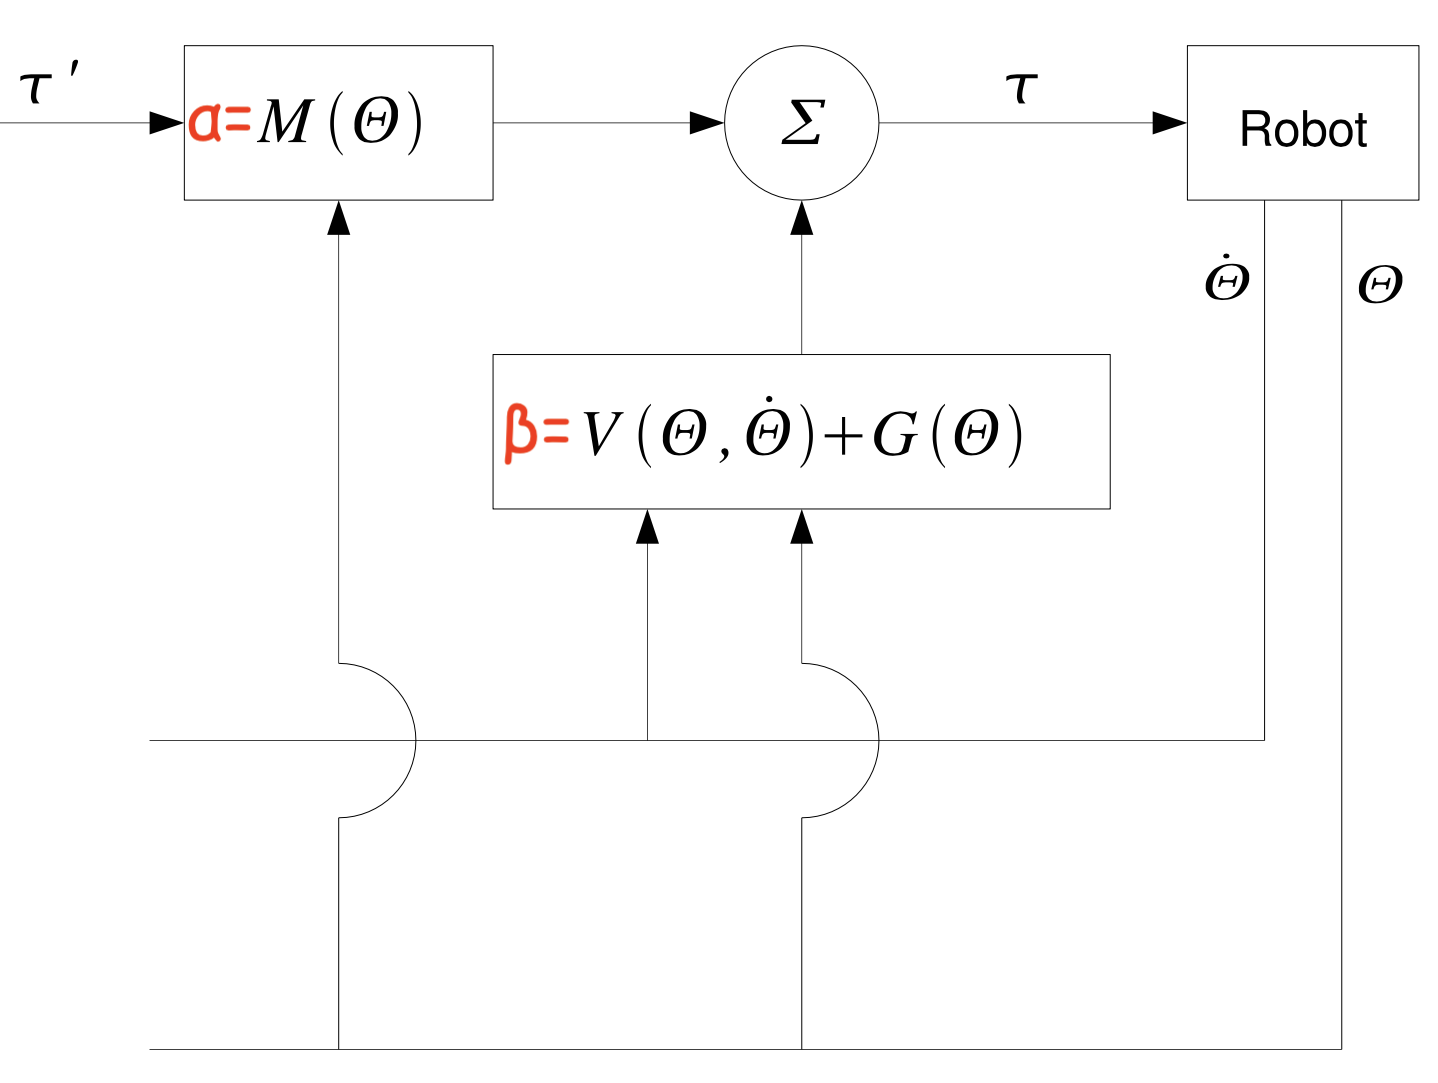
\includegraphics[width=5cm]{sections/imgs/8_controller_block_diagram.png}
	\end{minipage}
\end{center}





